

\documentclass[12pt]{article}
\usepackage{graphicx}


\begin{document}
\title{MON TITRE}
\author{Didi}
\maketitle

\newpage
\tableofcontents
\newpage


\section{Introduction}


\begin{figure}
    \centering
    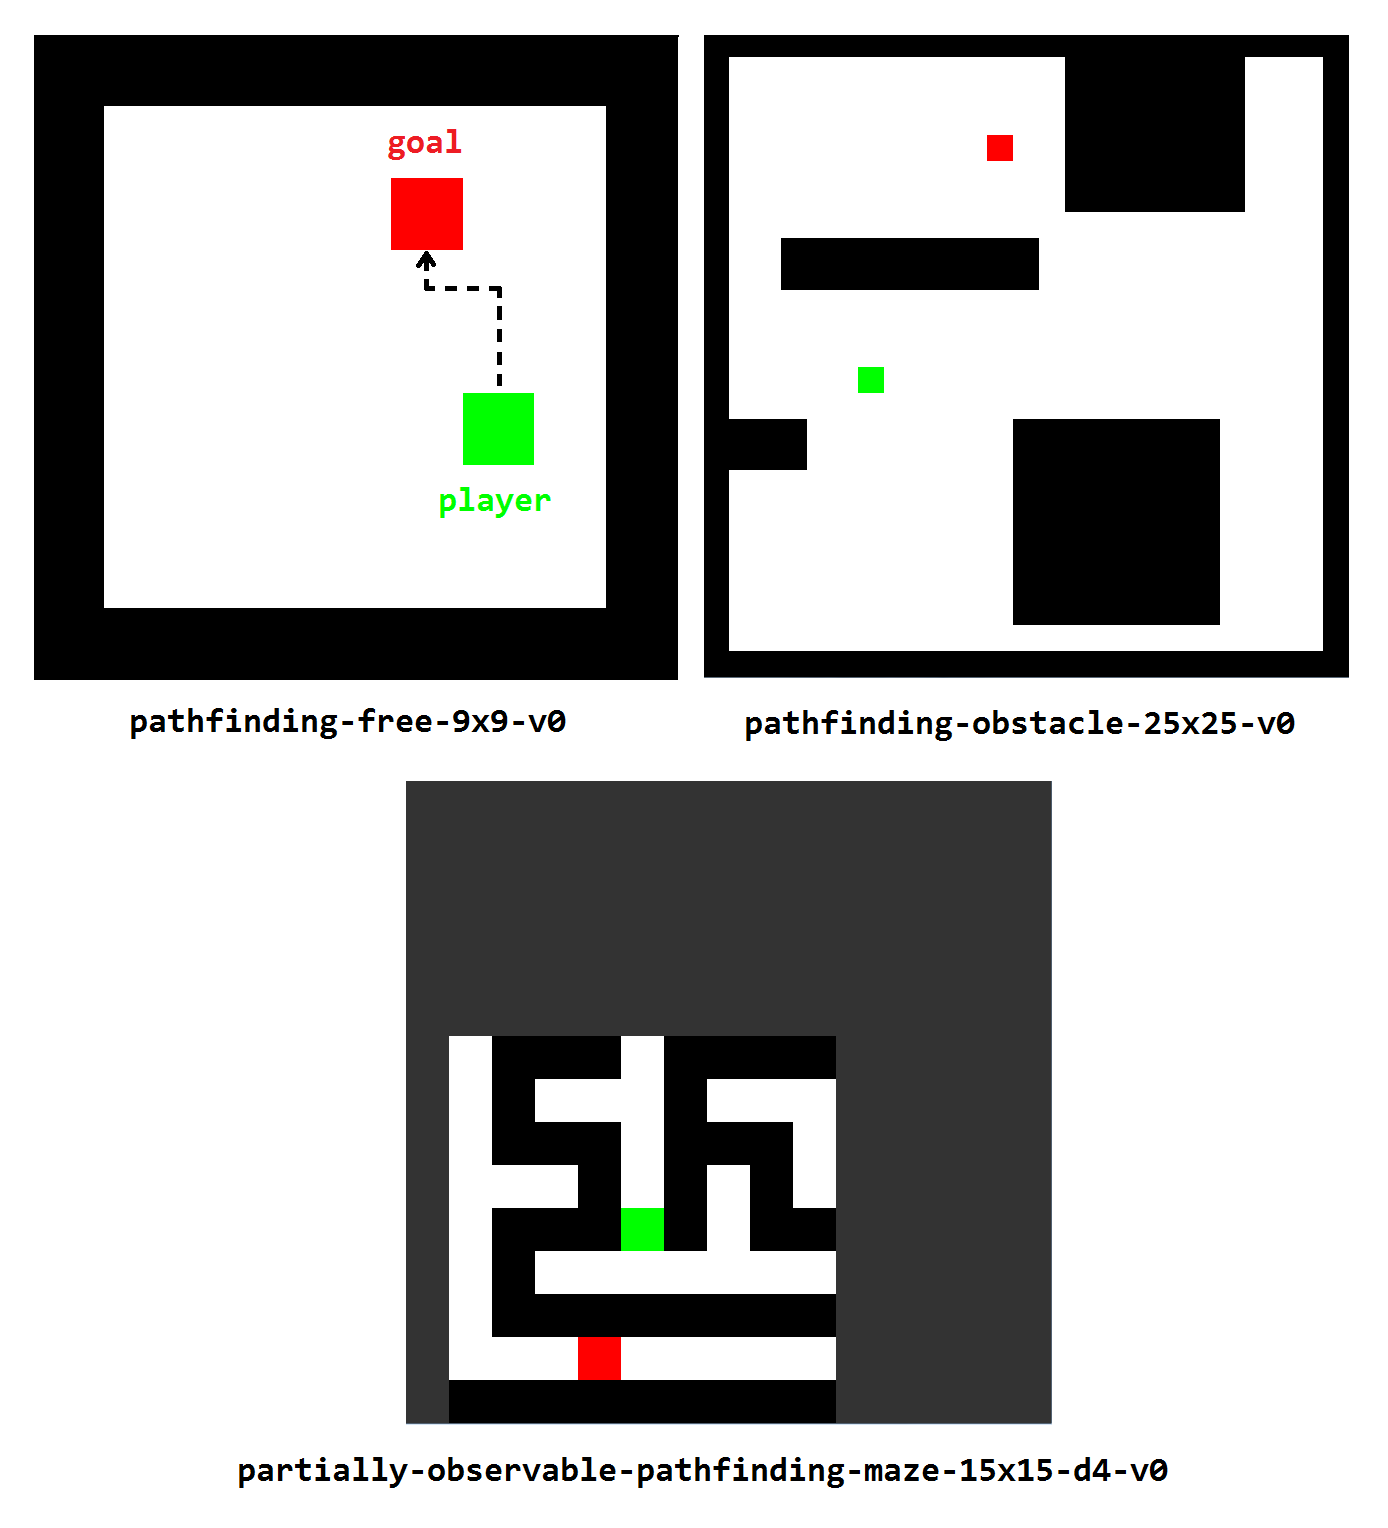
\includegraphics[width=0.5\textwidth]{env_examples.png}
    \caption{A boat.}
    \label{fig:boat1}
\end{figure}
\[
    f(x) = y
\]

Figure \ref{fig:boat1} shows a boat.


\section{Experiments}
Random citation \cite{DUMMY:1} embeddeed in text.
jhon = \cite{jhonlenon} mdr

arXiv:0706.1234


et le petit \cite{lol:1}

\newpage


\bibliography{paper} 
\bibliographystyle{ieeetr}


\end{document}

